\documentclass[aspectratio=169]{beamer}

\usepackage[utf8]{inputenc} % codificacao de caracteres
\usepackage[T1]{fontenc}    % codificacao de fontes
\usepackage[brazil]{babel}  % idioma

\usepackage{movie15}

\usetheme{Berlin}         % tema
\usecolortheme{seahorse}      % cores

\usefonttheme[onlymath]{serif} % fonte modo matematico
\usepackage{amsthm}

% Titulo
\title[\sc{Projeto e Análise de Algotimos}]{Meta Heuristica Simmulated Annealing para cortes 2D guilhotinados}
\author[Alano Martins Pinto]{Aeliton Silva e Alano Martins Pinto }
\institute{UECE - Universidade Estadual do Ceará} % opcional
\date{\today}


% Colocando numero de paginas no slide
\setbeamertemplate{footline}[frame number]

% Desativando os botoes de navegacao
\beamertemplatenavigationsymbolsempty

% Tela cheia\section{section1}

\hypersetup{pdfpagemode=FullScreen}

% Layout da pagina
\hypersetup{pdfpagelayout=SinglePage}

% Definicao de novos comandos
\providecommand{\sin}{} \renewcommand{\sin}{\hspace{2pt}\textrm{sen}}
\providecommand{\tan}{} \renewcommand{\tan}{\hspace{2pt}\textrm{tg}}
\newcommand{\R}{\mathbb{R}}

% Capa - requer o TikZ
\newcommand{\capa}{
    \begin{tikzpicture}[remember picture,overlay]
        \node at (current page.south west)
            {\begin{tikzpicture}[remember picture, overlay]
                \fill[shading=radial,top color=orange,bottom color=orange,middle color=red] (0,0) rectangle (\paperwidth,\paperheight);
            \end{tikzpicture}
          };
    \end{tikzpicture}
}


% Definicao de novos ambientes
\theoremstyle{Definition}
\newtheorem{defn}{Defini\c c\~ao}
\newtheorem{teo}[theorem]{Teorema}
\newtheorem{ex}[theorem]{Exemplo}
\newtheorem{eq}[theorem]{Equa\c c\~ao}


\usepackage{etoolbox}
\newcommand{\zerodisplayskips}{%
  \setlength{\abovedisplayskip}{0pt}%
  \setlength{\belowdisplayskip}{0pt}%
  \setlength{\abovedisplayshortskip}{0pt}%
  \setlength{\belowdisplayshortskip}{0pt}}
\appto{\normalsize}{\zerodisplayskips}
\appto{\small}{\zerodisplayskips}
\appto{\footnotesize}{\zerodisplayskips}
\begin{document}

\begin{frame}
\titlepage
\end{frame}

%\begin{frame}
%\tableofcontents
%\end{frame}

\begin{frame}
	\frametitle{Simulated Annealing}
	
		\begin{columns}
		\begin{column}{0.5\textwidth}
		   \begin{itemize}
		   		\item Técnica probabilistica x Espaço de busca
				\item Minimos Locais x Minimo Global
				\item Função objetiva
			\end{itemize}
		\end{column}
		\begin{column}{0.5\textwidth}  %%<--- here
    		\begin{figure}[h]
	   	 		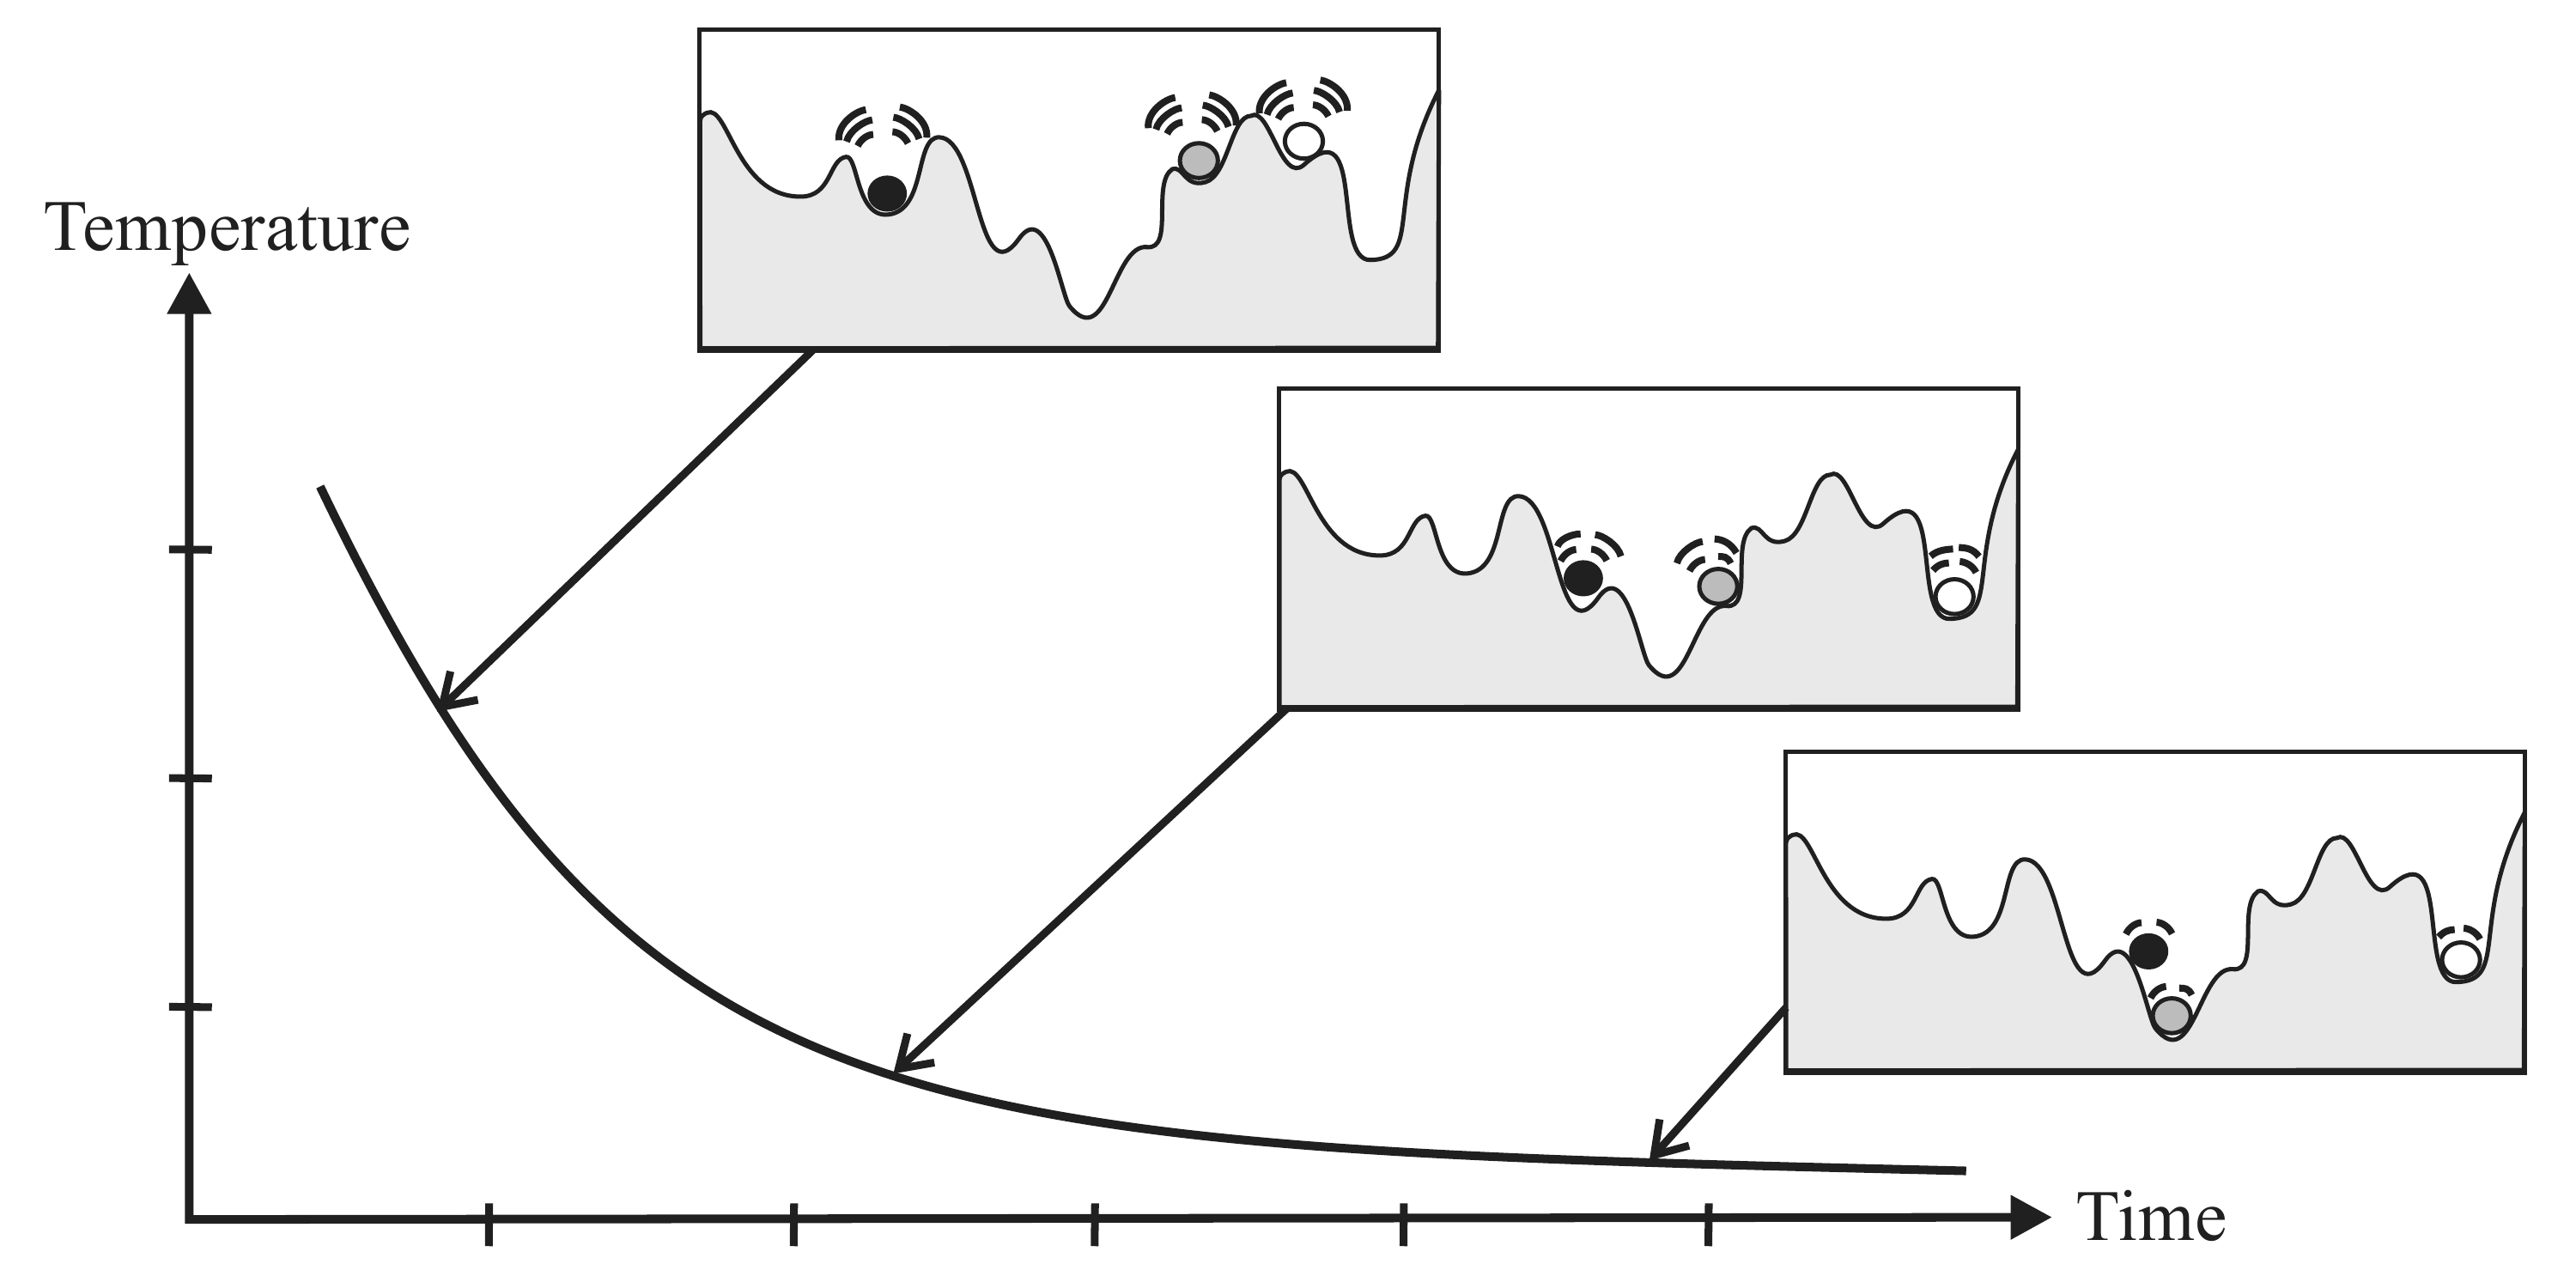
\includegraphics[width=7.5cm]{imagens/sa}
			    \caption{Mínimos}
	  		\end{figure}
		\end{column}
	\end{columns}
\end{frame}

\begin{frame}
	\frametitle{Resultados do S.A}
	
		\begin{columns}
		\begin{column}{0.5\textwidth}
		   \begin{itemize}
		   		\item Pertubação
				\item Vizinhança
				\item Interações
				\item Fator de Boltzmann
			\end{itemize}
		\end{column}
		\begin{column}{0.5\textwidth}  %%<--- here
    		\begin{figure}[h]
	   	 		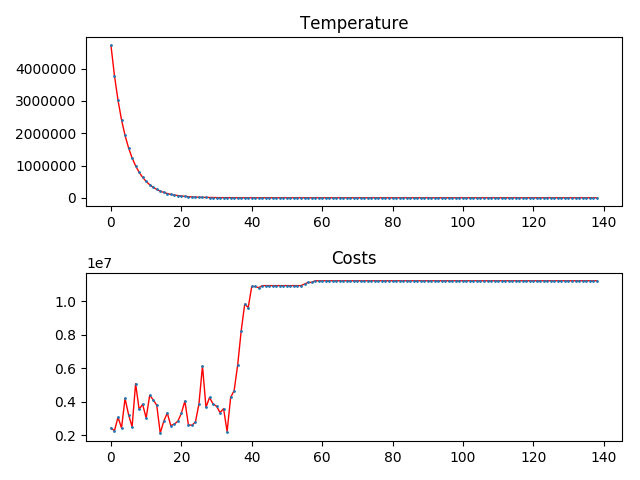
\includegraphics[width=7cm, height=4.8cm]{imagens/plot}
			    \caption{Função de custo x Temperatura}
	  		\end{figure}
		\end{column}
	\end{columns}
\end{frame}

\begin{frame}
	\frametitle{Resultados do corte guilhotinado}
	
		\begin{columns}
		\begin{column}{0.5\textwidth}
		   \begin{itemize}
		   		\item Repetição
				\item Solução inicial
			\end{itemize}
		\end{column}
		\begin{column}{0.5\textwidth}  %%<--- here
    		\begin{figure}[h]
	   	 		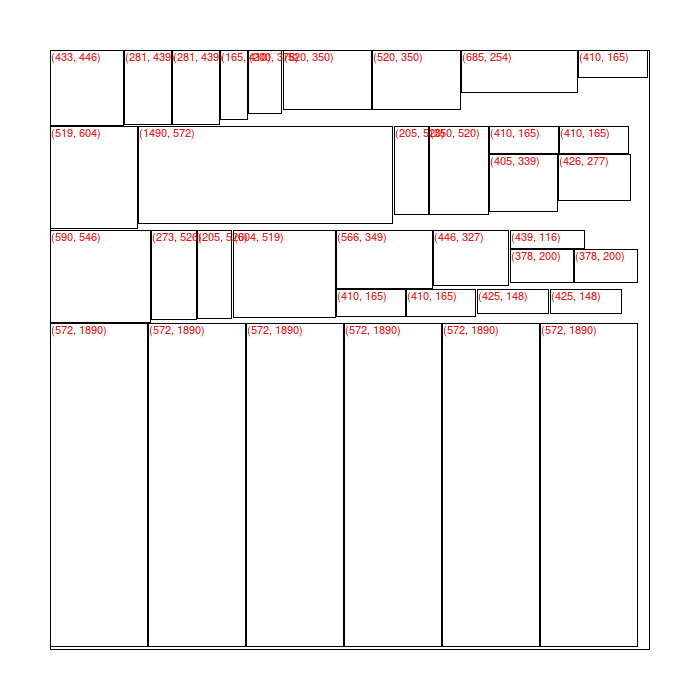
\includegraphics[width=7cm, height=4.8cm]{imagens/cut}
			    \caption{Função de custo x Temperatura}
	  		\end{figure}
		\end{column}
	\end{columns}
\end{frame}

\begin{frame}
Dúvidas?
\end{frame}

\begin{frame}
Obrigado
\end{frame}

\end{document}